\newcommand{\labtitle}{ECE/CS 5710/6710 - Lab 2}
%\newcommand{\labdate}{}
\newcommand{\labsubtitle}{CMOS Inverter - Physical Design}
\vlsiheader


\begin{center}
\LARGE\textbf{\labsubtitle} \\
	\large\textbf{Pre-lab Assignment:} Check for the date on Canvas. \\
	\large\textbf{Lab Report:} Check for the date on Canvas.
\end{center}
\section{Objectives}
The goal of this second lab is to teach you how to draw the layout of a CMOS inverter using the Skywater design kit. You will also learn how to verify your design through thse DRC and LVS steps and how to extract the layout parasitics for post-layout simulation purposes. For the DRC, LVS and PEX steps, you will use an industrial tool: Mentor Calibre\textsuperscript{\tiny\textregistered}.



\section{Pre-lab Assignment}
\begin{prelab}
Answer the following questions and submit a \textbf{.pdf} file through Canvas:
\begin{enumerate}
	\item What does DRC, LVS and PEX stand for? What are they used for?
	\item Draw the transistor schematic of a 2-input NAND gate and give its truth table.
	\item How are the transistor in a 2-input NAND gate usually sized? Justify your answer.
\end{enumerate}
	\vspace{-5mm}
\end{prelab}

\section{Introduction the the Tools}
In this lab, you will reuse Virtuoso\textsuperscript{\tiny\textregistered} for the layout as well as electrical simulations. You will also use Calibre\textsuperscript{\tiny\textregistered} is the suite for full-custom layout verification and parasitics extraction. Although it is coming from another vendor (Mentor, now part of Siemens), this tool is easily integrated into the Virtuoso\textsuperscript{\tiny\textregistered} environment.


\section{Lab Assignment}
\subsection{CMOS Inverter Layout Drawing}
In this part, you will learn how to draw the layout of the CMOS inverter. With this knowledge, you will then be able to draw the layout of more complex logic gates. To start this lab, launch Virtuoso\textsuperscript{\tiny\textregistered} from your \textit{virtuoso} subdirectory, as you did in the previous lab:
\begin{codeline}
	./start$\_$virtuoso.sh
\end{codeline}

\subsubsection{Layout Environment}
		\begin{remark}
	As explained in the previous lab, don't forget to check that in your inverter schematic view, the width of the $pmos$ is set to \textit{840nm} and not as a parameter, otherwise, you will have some issues when instantiating it in your layout.
\end{remark}
			\vspace{-8mm}
\begin{enumerate}
	
	\parbox[t]{\dimexpr\textwidth-\leftmargin}{%
		\begin{wrapfigure}[12]{r}{0.6\textwidth}
			\vspace{-0mm}
			\centering
			\vspace{-\baselineskip}
			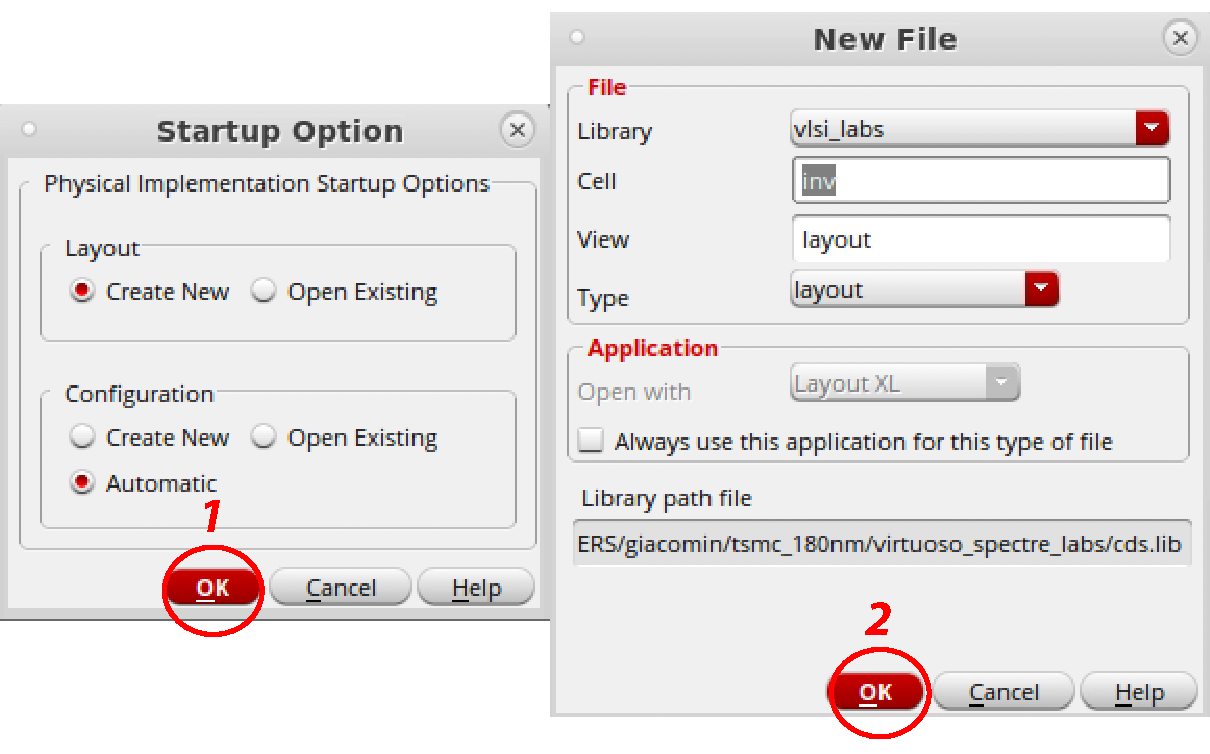
\includegraphics[scale=0.35]{figures/lab2_layout/layout_create.pdf}
			\caption{New layout view.}
			\label{fig_layoutfile}
		\end{wrapfigure}
		\item Create a new cellview for your inverter Layout. To do so, go to the open your inverter schematic and do: \textit{Launch - Layout XL ...}). Click OK on the first window. For the next window, select layout as the view name, and Layout XL as the desired application as indicated in Fig. \ref{fig_layoutfile} (the library and cell name will of course depend on what you chose earlier). \newline}
	
	
	\parbox[t]{\dimexpr\textwidth-\leftmargin}{%
		\begin{wrapfigure}[19]{r}{0.65\textwidth}
			\vspace{-0mm}
			\centering
			\vspace{-\baselineskip}
			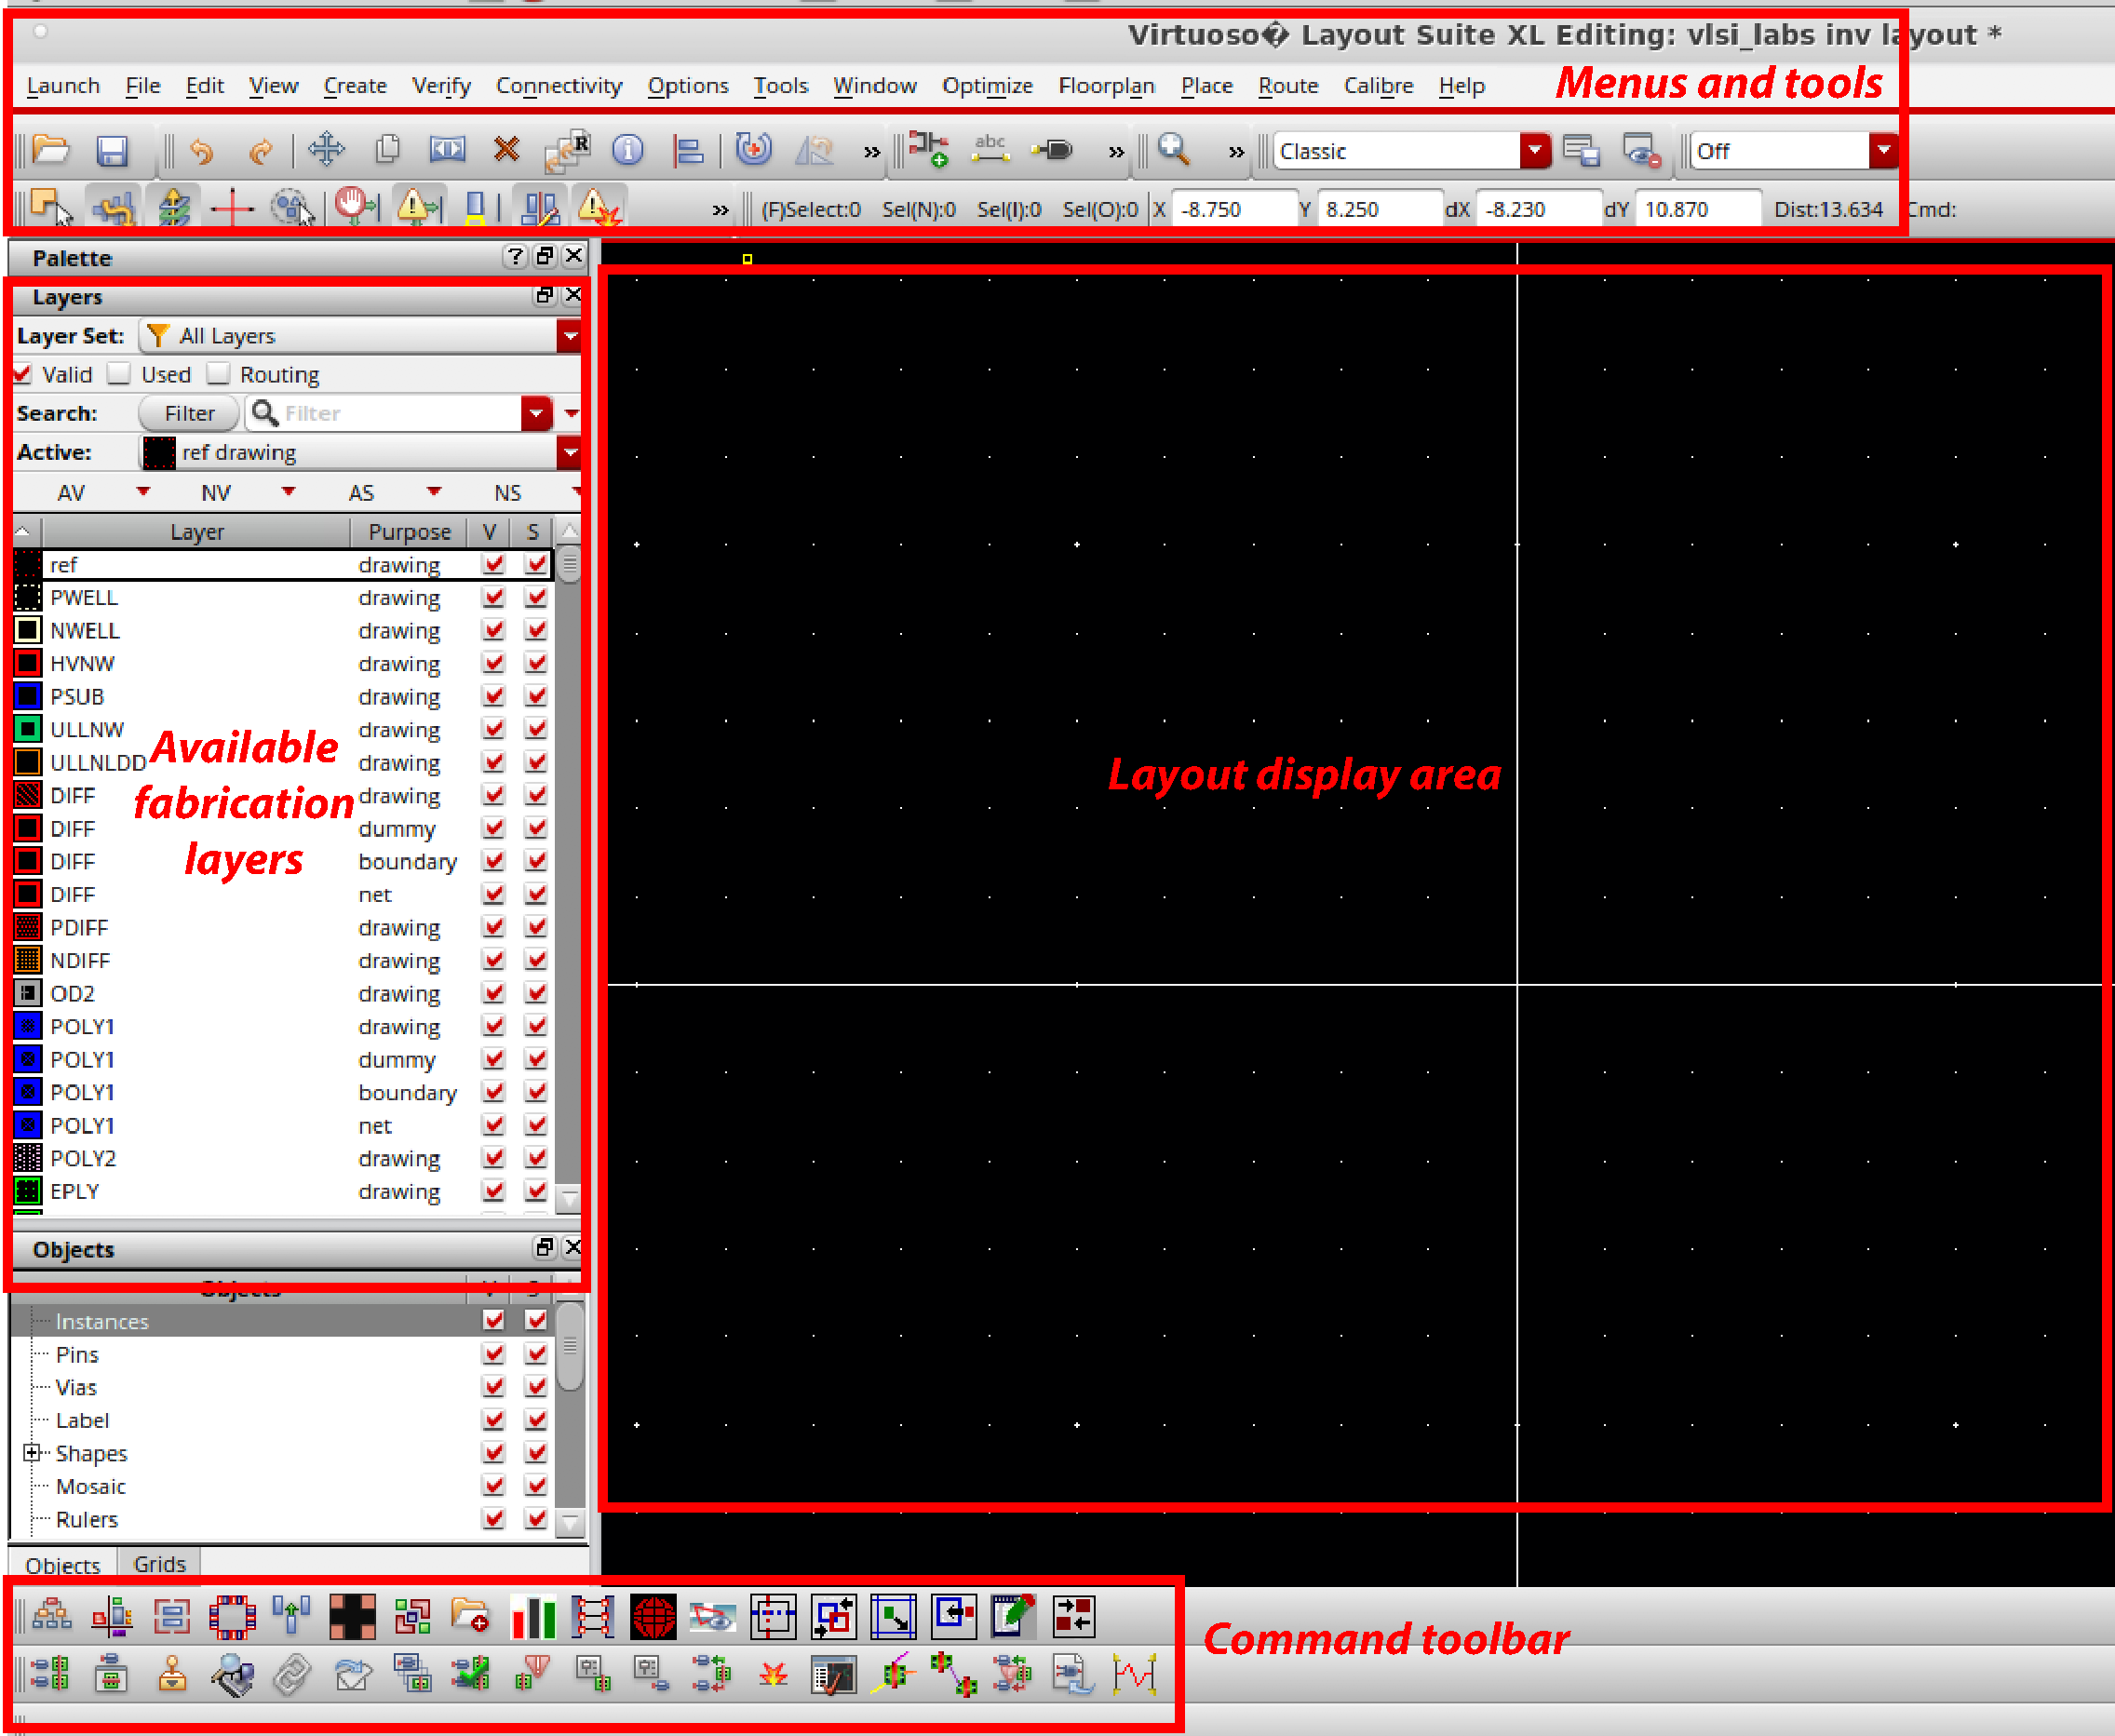
\includegraphics[scale=0.25]{figures/lab2_layout/layout.pdf}
			\caption{Layout XL window.}
			\label{fig_layoutwin}
		\end{wrapfigure}
		\item The Virtuoso\textsuperscript{\tiny\textregistered} Layout XL Editor window will appear. All available fabrication layers are listed in the layer sub-window on the left (Fig \ref{fig_layoutwin}). From here, you can select which current layers are visible (V) or selectable (S). You can also choose to only display the layers currently in use in your current layout but selecting \textit{Used}. Many useful commands can be found in the command toolbar below the layout display area. Most of the shortcuts to save, delete an instance, rotate a component, \textit{etc.} are located in the menus and tools area.
		As you saw in class, integrated circuits are manufactured through a lot of process steps and are composed by a large number of planar layers, stacked on top of each others. The layout is composed of the geometric shapes of each layers that corresponds to the actual pattern of those materials in your integrated circuit. Based on the layers you choose for your layout, precise masks will be generated during fabrication. This is why for a given layer (e.g. metal 1), several purpose layers are available (dummy, blockage, drawing).}
	\begin{remark}
		When closing your layout view and opening it again later, Layout L might be used instead. The only difference is that Layout XL contains more functionalities (such as instantiating the cells automatically, the ability to flatten your cells, \textit{etc.}). To switch, go to: \textit{Launch -> Layout XL}. 
	\end{remark}
	\clearpage
	As for the schematic view, lots of shortcuts are available in order to draw your layouts. The most important ones are given in Table. \ref{shortcuts}.

	\begin{table}[h!]
		\caption{Main Layout\textsuperscript{\tiny\textregistered} shortcuts.}
				\vspace{-2mm}
		\label{shortcuts}
		\centering
		\begin{tabular}{ |c| c|c| }
			\hline
			\textbf{Shortcut} & \textbf{Menu Access} &\textbf{Action}  \\ 
			\hline
			u & Edit -> Undo & Undo previous command \\  
			\hline
					c & Edit -> Copy & Copy selected instance(s)  \\  
			\hline
					m & Edit -> Move & Move selected instance(s)  \\  
			\hline
								s & Edit -> Stretch & Stretch selected layer  \\  
			\hline
			f & Window -> Fit All & Fit the entire design into the layout window  \\  
			\hline
			r & Create -> Rectangle & Create a rectangle shape  \\  
\hline
			i & Create -> Instance & Instantiate another design/layout in the current design  \\  
\hline
		o & Create -> Contact & Create a via/contact from the technology  \\  
\hline
		l & Create -> Label & Create a label for your pins  \\  
\hline
		q & Create -> Properties & Show the properties of selected instance  \\  
\hline
		k & Window -> Create ruler & Create a ruler to perform measurements  \\  
\hline
		ctrl+f & N/A & Shows the current level of hierarchy\\  
				& & All the instances in the lower levels are shown as red boxes  \\  
\hline
		shift+f & N/A & Shows all hierarchy levels. All the layers are shown  \\  
\hline
		\end{tabular}
	\end{table}
\end{enumerate}

\subsubsection*{Step 1: Transistors Instantiation}

	\begin{itemize}
\parbox[t]{\dimexpr\textwidth-\leftmargin}{%
	\begin{wrapfigure}[18]{r}{0.6\textwidth}
		\vspace{-6mm}
		\centering
		\vspace{-\baselineskip}
		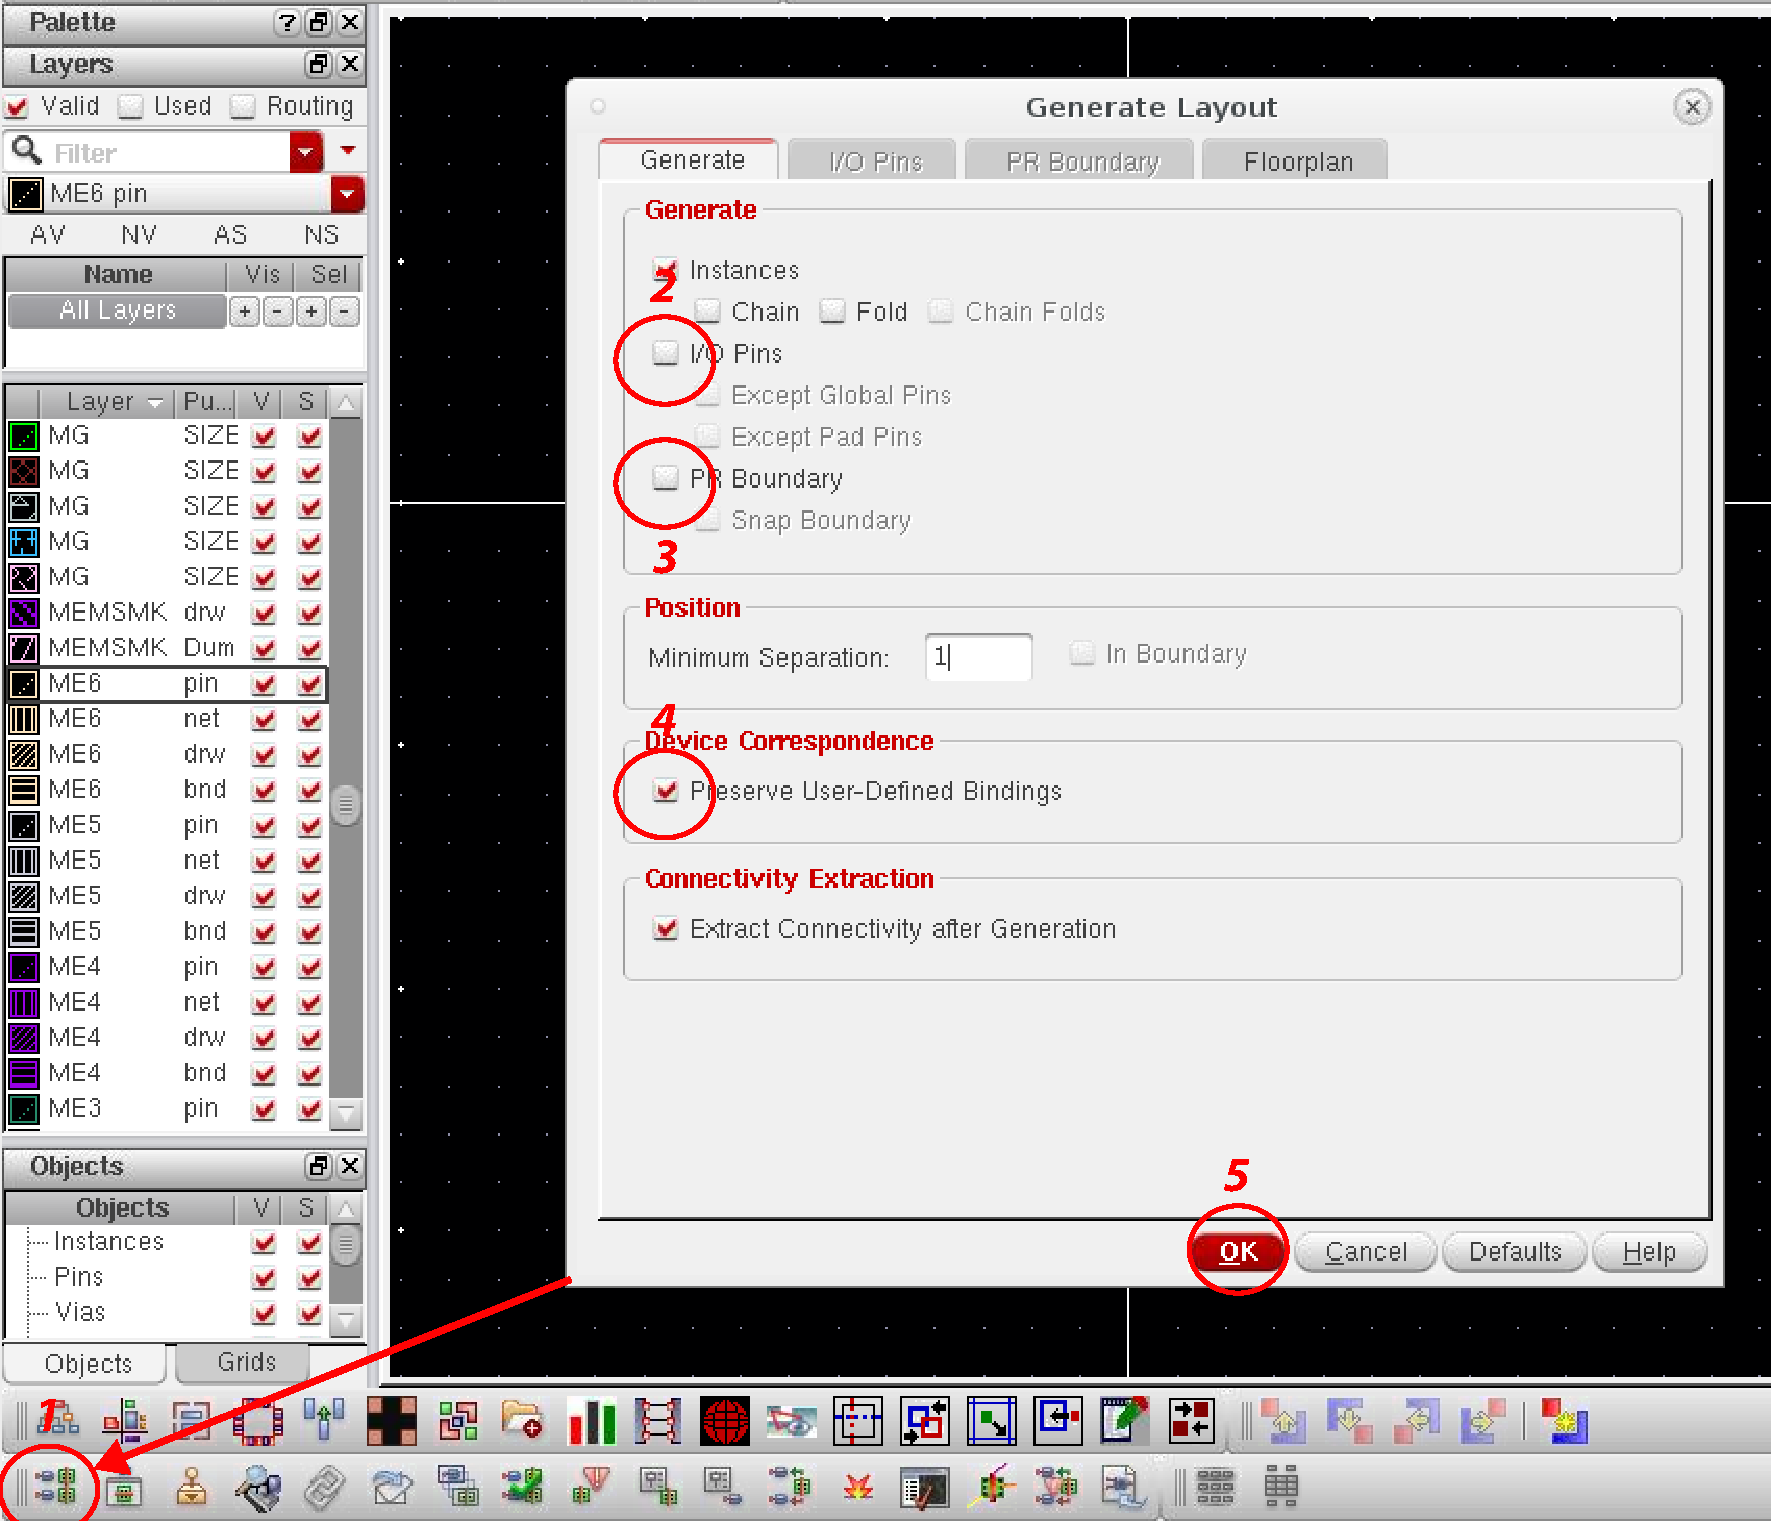
\includegraphics[scale=0.3]{figures/lab2_layout/layout_inst}
		\caption{Instantiating the transistors.}
		\label{layout_inst}
	\end{wrapfigure}
		\item Instantiate your transistors. To do so, from the layout editor Command Toolbar, choose Generate All From Source (as in Fig. \ref{layout_inst}), and set it up to generate only the instances and to preserve the device correspondence (mapping between the schematic and layout) and click OK.
		\item Your transistors should appear on the layout. \textbf{If all you can see is a red box with the transistors names, press \textbf{shift + f}}. It will allow you to display deeper levels of the hierarchy (here the several instances).}
	\end{itemize}


\begin{remark}
	Another way of instantiating your transistor is to press \textbf{i} and select the appropriate instance from one of the library, as you did for the schematic.
\end{remark}

\subsubsection*{Step 2: Placing your Transistors}
\parbox[t]{\dimexpr\textwidth-\leftmargin}{%
	\begin{wrapfigure}[24]{r}{0.32\textwidth}
		\vspace{-0mm}
		\centering
		\vspace{-\baselineskip}
		\includegraphics[scale=0.28]{figures/lab2/1}
				\caption{Using the ruler.}
	\end{wrapfigure}
	Now, let's place the $pmos$ transistor closer to the $nmos$. To do so, you need to move it vertically: press \textbf{m}, click on the $pmos$ transistor and move your mouse in the wanted direction. Here, we want the diffusion regions of our $nmos$ and $pmos$ to be distant by $.56 \mu m$. This distance is arbitrary for now, you don't have to necessary respect it for all your designs (the important distance to respect is the one between the power supply lines, which will bee explained in Step 6). To do so, we need to use some rulers:
	\begin{itemize}
		\item Press k to draw a ruler. To draw, select starting and ending points of the ruler by left-click after pressing k.
		\item You can always remove the existing rulers by pressing \textbf{Shift+k}.
		\item Use the ruler to check that the distance between both transistors is respected. If not, you need to move your transistors accordingly.
		\item Use the ruler again to make sure that the gate of both transistors are aligned. To do so, you can just place the ruler on the side of one of the gate and verify the alignment with the other gate.\end{itemize}
}


\subsubsection*{Step 3: Drawing the Poly-Silicon Gate Connection}
\parbox[t]{\dimexpr\textwidth-\leftmargin}{%
	\begin{wrapfigure}[28]{r}{0.5\textwidth}
		\vspace{-0mm}
		\centering
		\vspace{-\baselineskip}
		\includegraphics[scale=0.35]{figures/lab2/2}
		\caption{Poly-Silicon wire creation.}
		\label{layout_poly}
	\end{wrapfigure}
	Now, you need to connect the gate of the $nmos$ and $pmos$ together. To do so, you will draw a poly-silicon wire to connect both gates. 
	\begin{itemize}
		\item Select the poly-silicon layer on the drawing layers panel on the left by choosing $poly- drawing$, as depicted in Fig. \ref{layout_poly}.
		\item Press \textbf{p} and use the left mouse button to start and end the wire. For the starting point, select the top edge of the $nmos$ gate. For the ending point, select the bottom edge of the $pmos$. gate.\end{itemize}		\vspace{11mm}
}
	\begin{remark}
	It is possible to make the wire to break under a 90 degree angle if you use the left mouse button multiple times. However, at advanced technology nodes, it is generally harder to manufacture such kind of break lines due to the small size of the wires.
\end{remark}

\subsubsection*{Step 4: Placing the Poly-silicon to Metal1 Contact (Via)}
\begin{itemize}
	\item To draw the poly-silicon to metal 1 contact, multiple vias are necesary as there are multiple layers to traverse. Press \textbf{o} and select $PYL1_c$ as the Via Definition and then press $Hide$.
	\item Place your via on the poly-silicon wire as shown in Fig. \ref{layout_createvia}.
	\item This via will travel between the poly layer and the local interconnect layer. We must place one more via to get to the metal. Repeat the previous step with the $L1M1_c$ Definition and place it directly on top of the previous via.  \ref{layout_createvia}.
	\begin{figure}[!h]
		\centering
		\includegraphics[scale=0.32]{figures/lab2/3}
		\caption{Poly-silicon-Metal1 via creation.}
		\label{layout_createvia}
	\end{figure}
	
\end{itemize}


\subsubsection*{Step 5: Creating the Metal 1 Wire}
\parbox[t]{\dimexpr\textwidth-\leftmargin}{%
	\begin{wrapfigure}[28]{r}{0.5\textwidth}
		\vspace{-6mm}
		\centering
		\vspace{-\baselineskip}
		\includegraphics[scale=0.32]{figures/lab2/4}
		\caption{Local interconnect wire creation.}
		\label{layout_metal1}
	\end{wrapfigure}
	Now, you need to connect the drain of your $nmos$ and $pmos$ together to define your inverter output. To do so:
	\begin{itemize}
		\item Select the first level local interconnect layer on the drawing layers panel on the left by choosing $li1- drawing$. \ref{layout_metal1}.
		\item Press \textbf{p} and use the left mouse button to start and end the wire. For the starting point, select the top edge of the $nmos$ drain metal 1 area. For the ending point, select the top edge of the $pmos$ drain metal 1 area.\end{itemize}
}

\subsubsection*{Step 6: Creating the Metal 1 VDD and GND Supply Lines}


\parbox[t]{\dimexpr\textwidth-\leftmargin}{%
	\begin{wrapfigure}[28]{r}{0.13\textwidth}
		\vspace{-6mm}
		\centering
		\vspace{-\baselineskip}
			\includegraphics[scale=0.33]{figures/lab2/5}
\caption{Standard cell height requirements.}
\label{spacing}
	\end{wrapfigure}
	Now, you need to connect the drain of your $nmos$ and $pmos$ together to define your inverter output. To do so:
		\begin{itemize}
	\item Select MET1-drawing as a layer. Press \textbf{r} and draw a rectangle of random dimensions, as depicted in Fig. \ref{layout_rectangle}. Then select the metal 1 rectangle, click on \textbf{q} and change its width and height to $4.6 \mu m$ and $0.29 \mu m$ respectively.
			\begin{remark}
		You will learn later that integrated circuits are composed of many rows where each row contains standard cells (INV, MUX, \textit{etc}). \textcolor{red}{\textbf{Therefore, all of your standard cells need in this lab and the next ones need to have the same height}. For this technology, you need to ensure your supply line have an height of  $0.29 \mu m$. The standard cell height being $2.72kk \mu m$, you need to check that the spacing between both metal supply lines is $2.43 \mu m$, as depicted in Fig. \ref{spacing}.} In addition, the width of your cell needs to be a multiple of $4.6 \mu m$. Since the inverter is thinner than this, we chose to use $4.6 \mu m$.
	\end{remark}
	\item Place the metal 1 rectangle on top of the $pmos$ transistor, with a distance of $0 \mu m$ from the $NWELL$ layer as shown Fig. \ref{layout_rectangle}.
	\item Place a similar rectangle on the bottom of the $nmos$. To do so, press \textbf{c} (for copy), select the first metal 1 rectangle and move the second rectangle on the bottom, with a distance of $0.06 \mu m$ from the $nsdm$ (red) layer.. 
\end{itemize}
}

	\begin{figure}[!h]
		\centering
		\includegraphics[scale=0.33]{figures/lab2/6}
		\caption{Metal 1 rectangle creation and placement for the power supply lines.}
		\label{layout_rectangle}
	\end{figure}


\subsubsection*{Step 7: Finishing the Metal Connections}

\parbox[t]{\dimexpr\textwidth-\leftmargin}{%
	\begin{wrapfigure}[18]{r}{0.4\textwidth}
		\vspace{-6mm}
		\centering
		\vspace{-\baselineskip}
		\includegraphics[scale=0.25]{figures/lab2/7}
				\caption{Connecting the terminals to the supply metal lines.}
	\end{wrapfigure}
	Connect the source of the $nmos$ and $pmos$ to the appropriate power supply lines through the local interconnect layer. To do so:
	\begin{itemize}
		\item Press \textbf{p} and draw a line from the source of the $pmos$ to the $vdd$ power line. Double-click to confirm the line.
		\item Place a via that will connect the local interconnect and the metal 1 layers.
		\item Repeat the previous steps to connect the source of the $nmos$ to $gnd$.\end{itemize}
}


		\vspace{26mm}
\subsubsection*{Step 8: Creating the Bulk Taps}
\begin{itemize}
	\item Now, we need to create to connect the bulk of the $nmos$ and $pmos$ to $VDD$ and $GND$ respectively.
	\item Extend some local interconnect lines to the left from the vdd and ground pins on the pmos and nmos.
	\item At the end of each line, place a via that connects the tap and local interconnect layers (TPL1$\_$C).
	\item The VDD tap will need to be surrounded by a rectangle of the nsdm layer, and a rectangle of the nwell layer.
	\item The GND tap will need to be surrounded by a rectangle of the psdm layer.

	\begin{figure}[!h]
		\centering
		\includegraphics[scale=0.33]{figures/lab2/8}
						\caption{Creating the bulk taps.}
	\end{figure}
\end{itemize}

\subsubsection*{Step 9: Creating the Pins/Ports}

\parbox[t]{\dimexpr\textwidth-\leftmargin}{%
	\begin{wrapfigure}[20]{r}{0.6\textwidth}
		\vspace{-0mm}
		\centering
		\vspace{-\baselineskip}
		\includegraphics[scale=0.33]{figures/lab2/9}
		\caption{Creating Pins.}
		\label{pins}
	\end{wrapfigure}
	Now, we need to create the pins so the LVS tool will be able to compare the schematic and the layout connectivity.
	\begin{itemize}
		\item We need a pin for VDD, GND, A, and Z (Z will also need a via to metal first).
		\item To create a pin, go to Create -> Pin in the toolbar.
		\item Assure the name is the same as the net it will be place on, select rectange, and assure the io and signal types are correct. (In this example, "A" is an input signal.)
		\item Click $Hide$, and draw the pin rectangle over the targeted via (assure met1 - pin in the selected layer)
		\item Click on $Hide$ and place them on your layout.
		\item In this specific case with the "A" pin, there is only a metal via beneath the pin. You will need to place a metal 1 - drawing layer rectangle beneath the pin for it to be recognized. \ref{pins}\end{itemize}
}

\subsubsection*{Step 10: Labeling}

\parbox[t]{\dimexpr\textwidth-\leftmargin}{%
	\begin{wrapfigure}[20]{r}{0.6\textwidth}
		\vspace{-0mm}
		\centering
		\vspace{-\baselineskip}
		\includegraphics[scale=0.33]{figures/lab2/10}
		\caption{Final inverter layout.}
		\label{final_layout}
	\end{wrapfigure}
	Finally all the ports need to be labeled.
	\begin{itemize}
		\item Select the MET1-pin layer and go to: Create -> Label... (or press l).
		\item Write in a pin name (or all of them separated by spaces). They need to match the pins of your schematic.
		\item Set the label size to something resonable (~.3)
		\item Click on $Hide$ and place them on your layout
		\item Assure the name is the same as the net it will be place on, select rectange, and assure the io and signal types are correct. (In this example, "A" is an input signal.)
		\item Click $Hide$, and draw the pin rectangle over the targeted via (assure met1 - pin in the selected layer)
		\item Click on $Hide$ and place them on your layout.
		\item Your layout should be (mostly) complete now and look like Fig. \ref{final_layout}. In the next part, you will verify it and correct the potential errors.\end{itemize}
}

\clearpage
\subsection{CMOS Inverter Layout Verification}
In this part, you will learn how to perform all the necessary layout verification steps (DRC and LVS) and how to extract the parasitic values from your layout (PEX).
\subsubsection{DRC Verification}
Even if you followed the previous steps for the layout of your inverter, you will probable get some DRC errors. ($Hint$: 3 of these errors can be solved by extending the $diff$, $poly$, and $li1$ layers of the nfet downwards $.06 \mu m$)The goal of this part is for you to understand those errors and to correct those by yourself. To perform the DRC step:
	\begin{enumerate}

	\begin{figure}
		\vspace{-0mm}
		\centering
		\vspace{1cm}
		\includegraphics[scale=0.2]{figures/lab2_layout/drc_main}
		\caption{Calibre nmDRC main window.}
		\label{fig_drcmain}
	\end{figure}
	\parbox[t]{\dimexpr\textwidth-\leftmargin}{%
		\item Launch the Calibre DRC tool: from the layout view: \textit{Calibre -> Run nmDRC…}.
		\item The Calibre nmDRC window now appears (Fig. \ref{fig_drcmain}). Normally, you should not have to modify anything on the nmDRC window except for setting the runset file to:
		
		\begin{codeline}
			/uusoc/facility/cad$\_$common/skywater-src-nda/s8/V2.0.1/DRC/Calibre/s8$\_$drc$\_$runset
		\end{codeline}
		
		\item You can take a quick look at the different DRC settings to understand better how the tool work. For instance, if you click on \textit{Rules}, you can see what calibre rule file is selected to check your layout, as well as the different layers derivations.		\vspace{2mm}
}

\parbox[t]{\dimexpr\textwidth-\leftmargin}{%
	\begin{wrapfigure}[14]{r}{0.6\textwidth}
		\vspace{-0mm}
		\centering
		\vspace{-\baselineskip}
		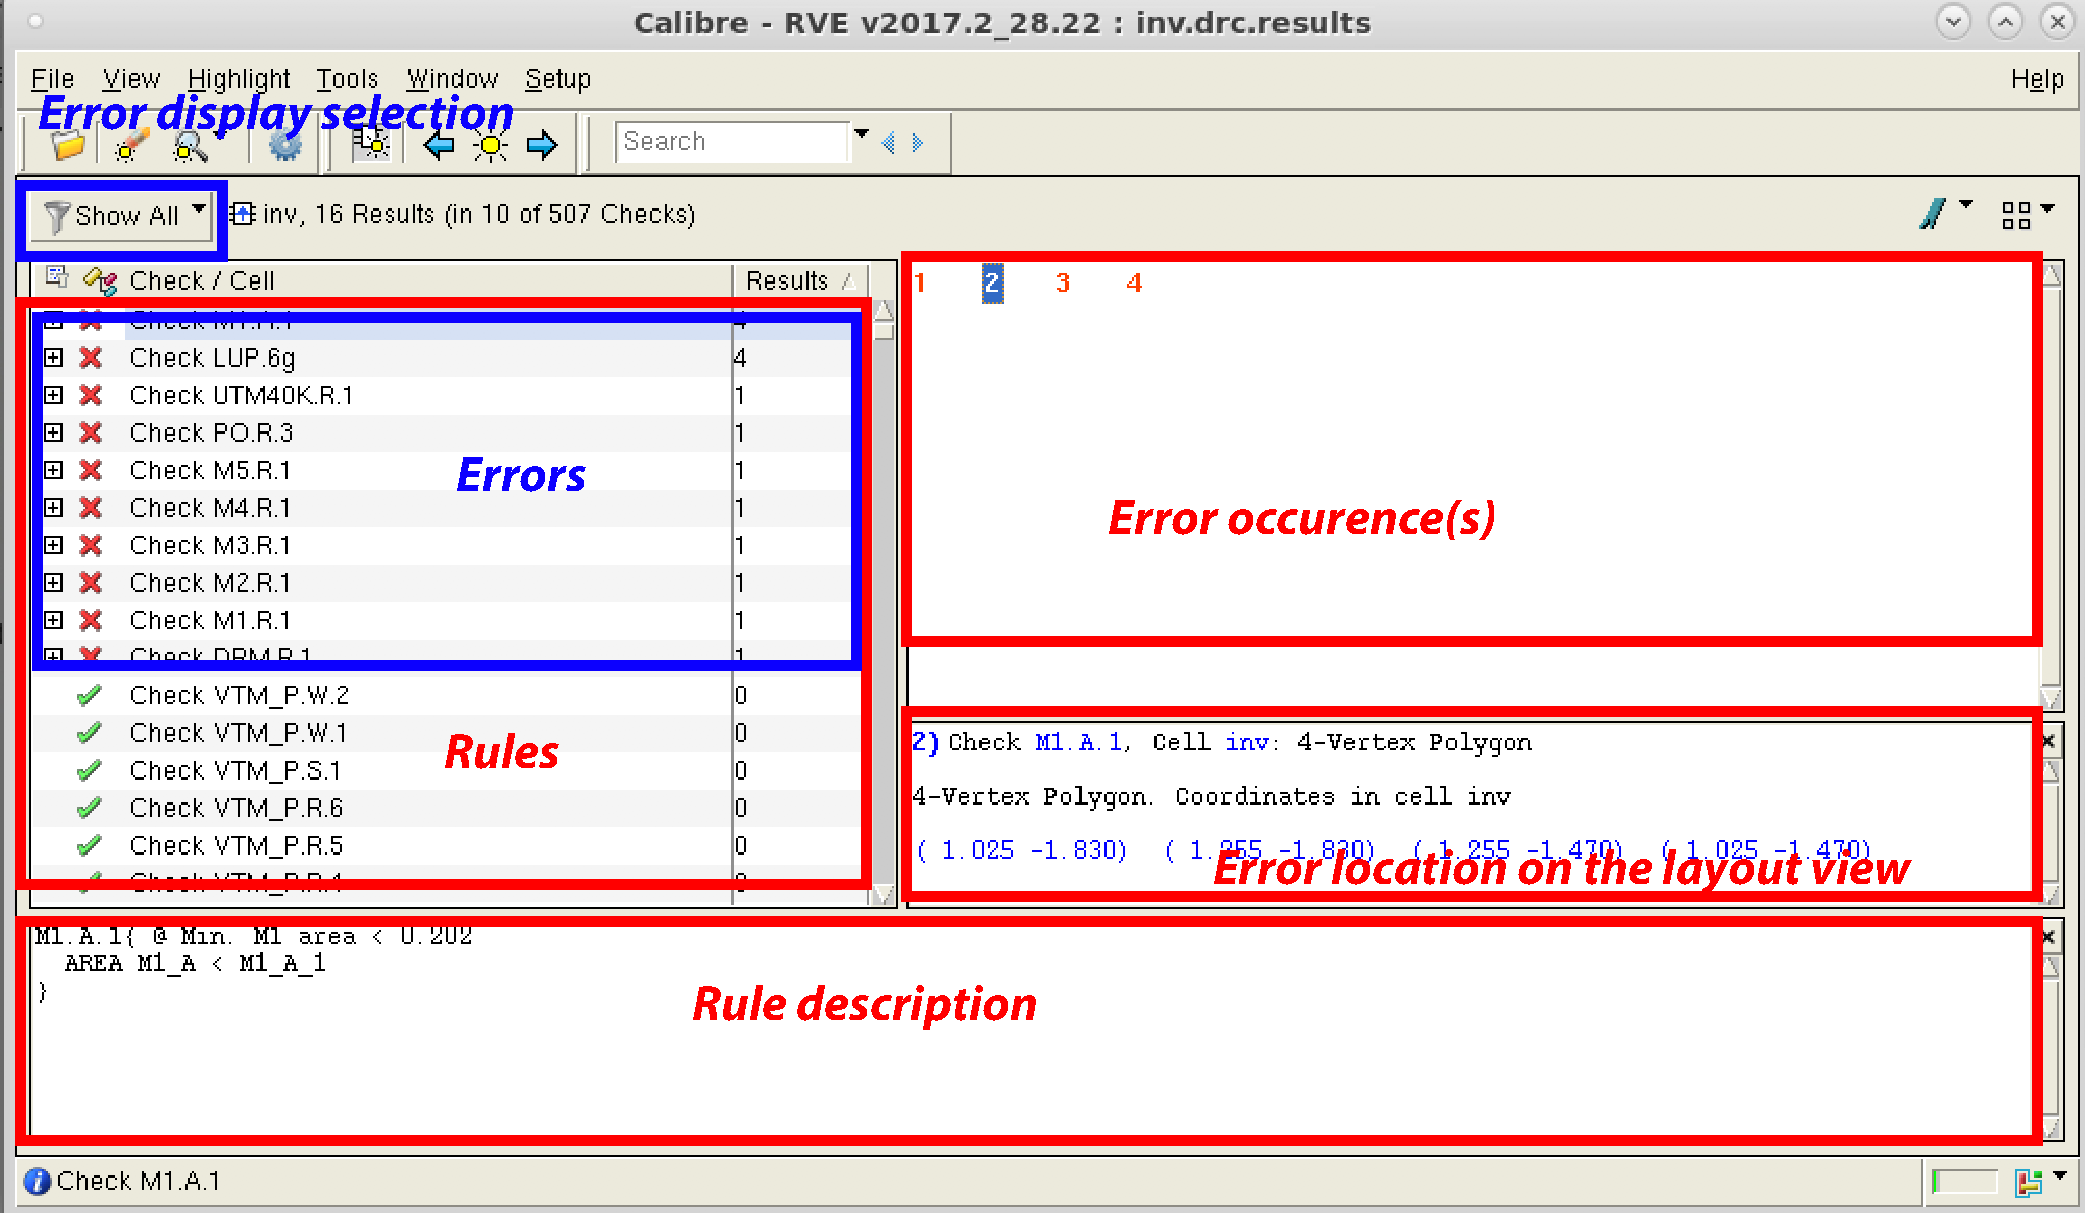
\includegraphics[scale=0.28]{figures/lab2_layout/drc_verif.pdf}
\caption{DRC result window}
\label{fig_drcverif}
	\end{wrapfigure}
	\item Then Click on Run DRC, wait a little bit and the potential DRC errors will be displayed. As shown in Fig. \ref{fig_drcverif}, a new window should appear. On the left pane are listed all the different rules. You can click on $Results$ to order them. If some rules have a red cross in front of them, it means your design does not respect some of the foundry rules (the goal is then to only have green symbol in front of every rules, otherwise, the foundry will not be able to manufacture your design). The rule description tells you what the rule require to be enforced. In this example, it says that the minimum metal 1 area should be at least $0.202 \mu m^2$. The error occurrence tells you how many occurrence of the same error you have in your design. The other pane tells you where the error is located. If you want to directly locate the error on your layout view, you can double click on the error number in the error occurrence pane (1 2 3 4 in Fig. \ref{fig_drcverif}). Once this error is corrected, you can go back to the DRC results window, select another error, locate it and so on and so forth.\vspace{2mm}
}

	\item Once you have corrected some errors, go back to the Calibre nmDRC window, click on Run DRC and check again how many error you get. You need to repeat this step until there is no DRC error at all in your design. You don't have to correct all the errors at once before running DRC again. 
	
	\begin{remark}
		It is often a good practice to correct some errors and run the tool again to see your progress (sometimes, by correcting some errors you might create new ones so it's better to go step by step). \newline
		When closing the DRC window, you will be asked if you want to save your changes to the runset file. Select \textit{No} and do the same when closing the LVS and PEX tools in the rest of the lab.
	\end{remark}
	
\end{enumerate}

\subsubsection{LVS Verification}

\begin{figure}
	\vspace{-0mm}
	\centering
	\vspace{1cm}
	\includegraphics[scale=0.25]{figures/lab2_layout/lvs_main}
	\caption{Calibre nmLVS main window.}
	\label{fig_lvsmain}
\end{figure}

\parbox[t]{\dimexpr\textwidth-\leftmargin}{%
	To perform the LVS step:
	\begin{enumerate}
		\item Launch the Calibre LVS tool: from the layout view: \textit{Calibre -> Run nmLVS…}.
		\item When the \textit{Load Runset File} window appears, browse and select: 
		\item The Calibre nmLVS window now appears (Fig. \ref{fig_lvsmain}). As for the DRC, you should not have to modify anything on the nmLVS window except setting the LVS runset file to:
		
		\begin{codeline}
			/uusoc/facility/cad$\_$common/skywater-src-nda/s8/V2.0.1/LVS/Calibre/s8$\_$lvs$\_$runset
		\end{codeline}

		\item Then Click on Run LVS, wait a little bit and the potential LVS errors will be displayed. A new LVS result window should appear. If your layout is correct, you should see the green smiley and icons as shown in Fig. \ref{fig_lvsverif}. If not, it means you have some errors. On the left pane are listed the different errors as follows:
\end{enumerate}}

%		\textit{$/research/ece/lnis-teaching$\newline$/5710\_6710/Runsets/$\newline$tsmc180nm\_lvs\_runset$} and click OK. The runset will define the settings of the LVS tools (in the same manner as before for the DRC). 

%\begin{figure}[!h]
%	\centering
%		\includegraphics[scale=0.4]{figures/drcrunset}
%\caption{LVS runset selection.}
%\label{fig_lvsrunset}
%\end{figure}
\begin{itemize}	
\parbox[t]{\dimexpr\textwidth-\leftmargin}{%
	\begin{wrapfigure}[24]{r}{0.62\textwidth}
		\vspace{0mm}
		\centering
		\vspace{-\baselineskip}
	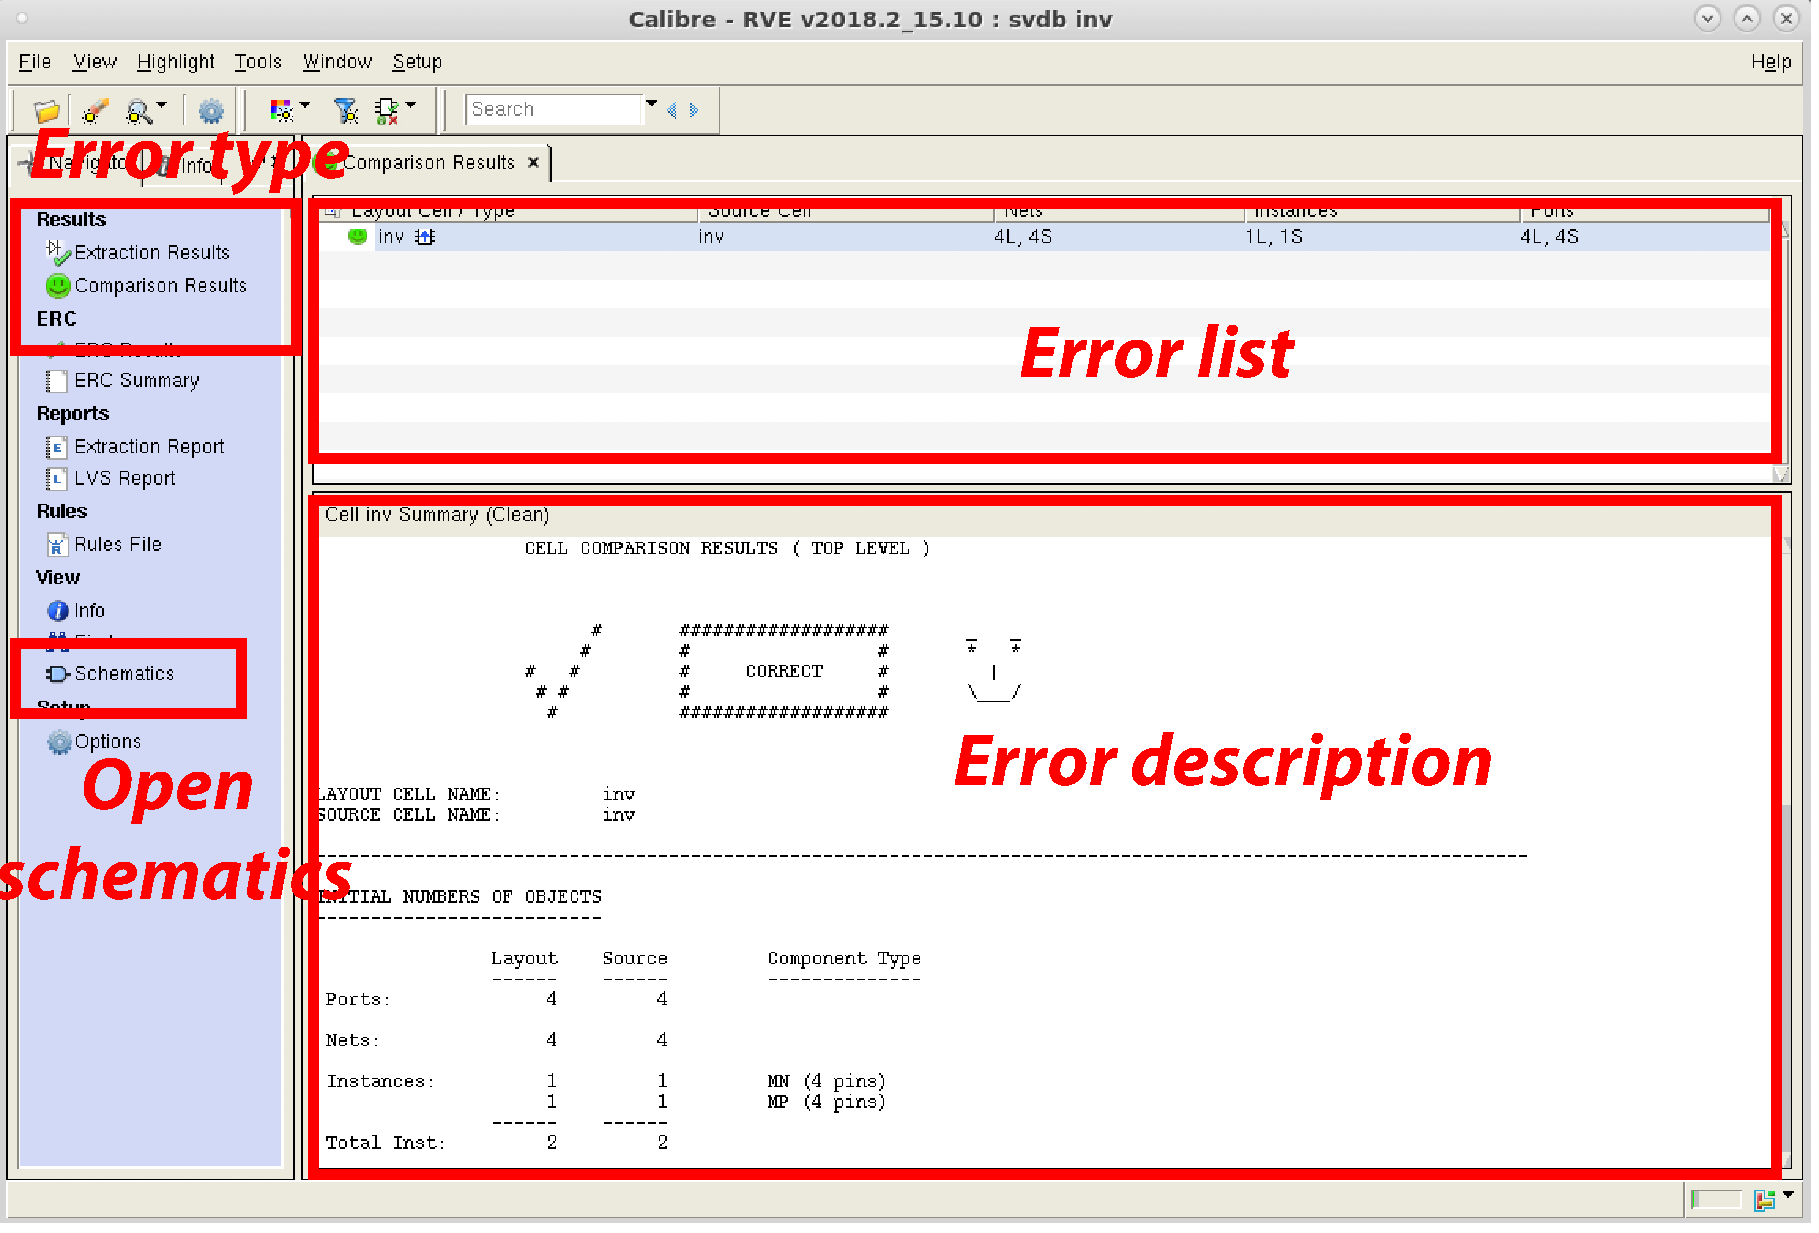
\includegraphics[scale=0.3]{figures/lab2_layout/lvs_verif}
\caption{LVS result window.}
\label{fig_lvsverif}
	\end{wrapfigure}
	\item \textbf{Extraction results} will list the pin related errors. For instance, if you define the same pin on two different nets, or if your design is missing the power supply or the ground pin, errors will be reported. 
	\item \textbf{Comparison results} will list the mismatches between your schematic and your layout. For instance, if you forget to connect the source of the \textit{nmos} of your inverter to the ground, an error will be reported.}
\end{itemize}


		\vspace{2mm}
To help you correct some LVS errors, Fig. \ref{fig_lvs_bad} shows an inverter design with some errors. In case you have some extraction errors, click on \textit{Extraction Results} and you will see the different errors in the error list. In Fig. \ref{fig_lvs_bad} (a), the error is caused by an absence of the power supply pin. To display the comparison errors, click on \textit{Comparison Results}. In Fig. \ref{fig_lvs_bad} (b), there are two errors: the nets $A$ and $Z$ can not be found in the layout since the pins have not been specified either. In some cases, an error could be caused by a bad connection (i.e. the input and output of the inverter could be connected together by a metal line). In the error description panel, you can click on the net names ($A$ and $Z$ in this case) and the associated net will be highlighted on either the source (schematic) or layout of your design. 

\begin{remark}
	Sometimes, it can be helpful to click on \textit{Schematics} on the LVS result window. It will open both the schematic of your design and the equivalent schematic of your layout. From here, you can visualize the difference and correct them. \newline
	As before, it is a good practice to correct some errors and run the tool again to see your progress.
\end{remark}

\begin{figure}[!h]
	\centering
	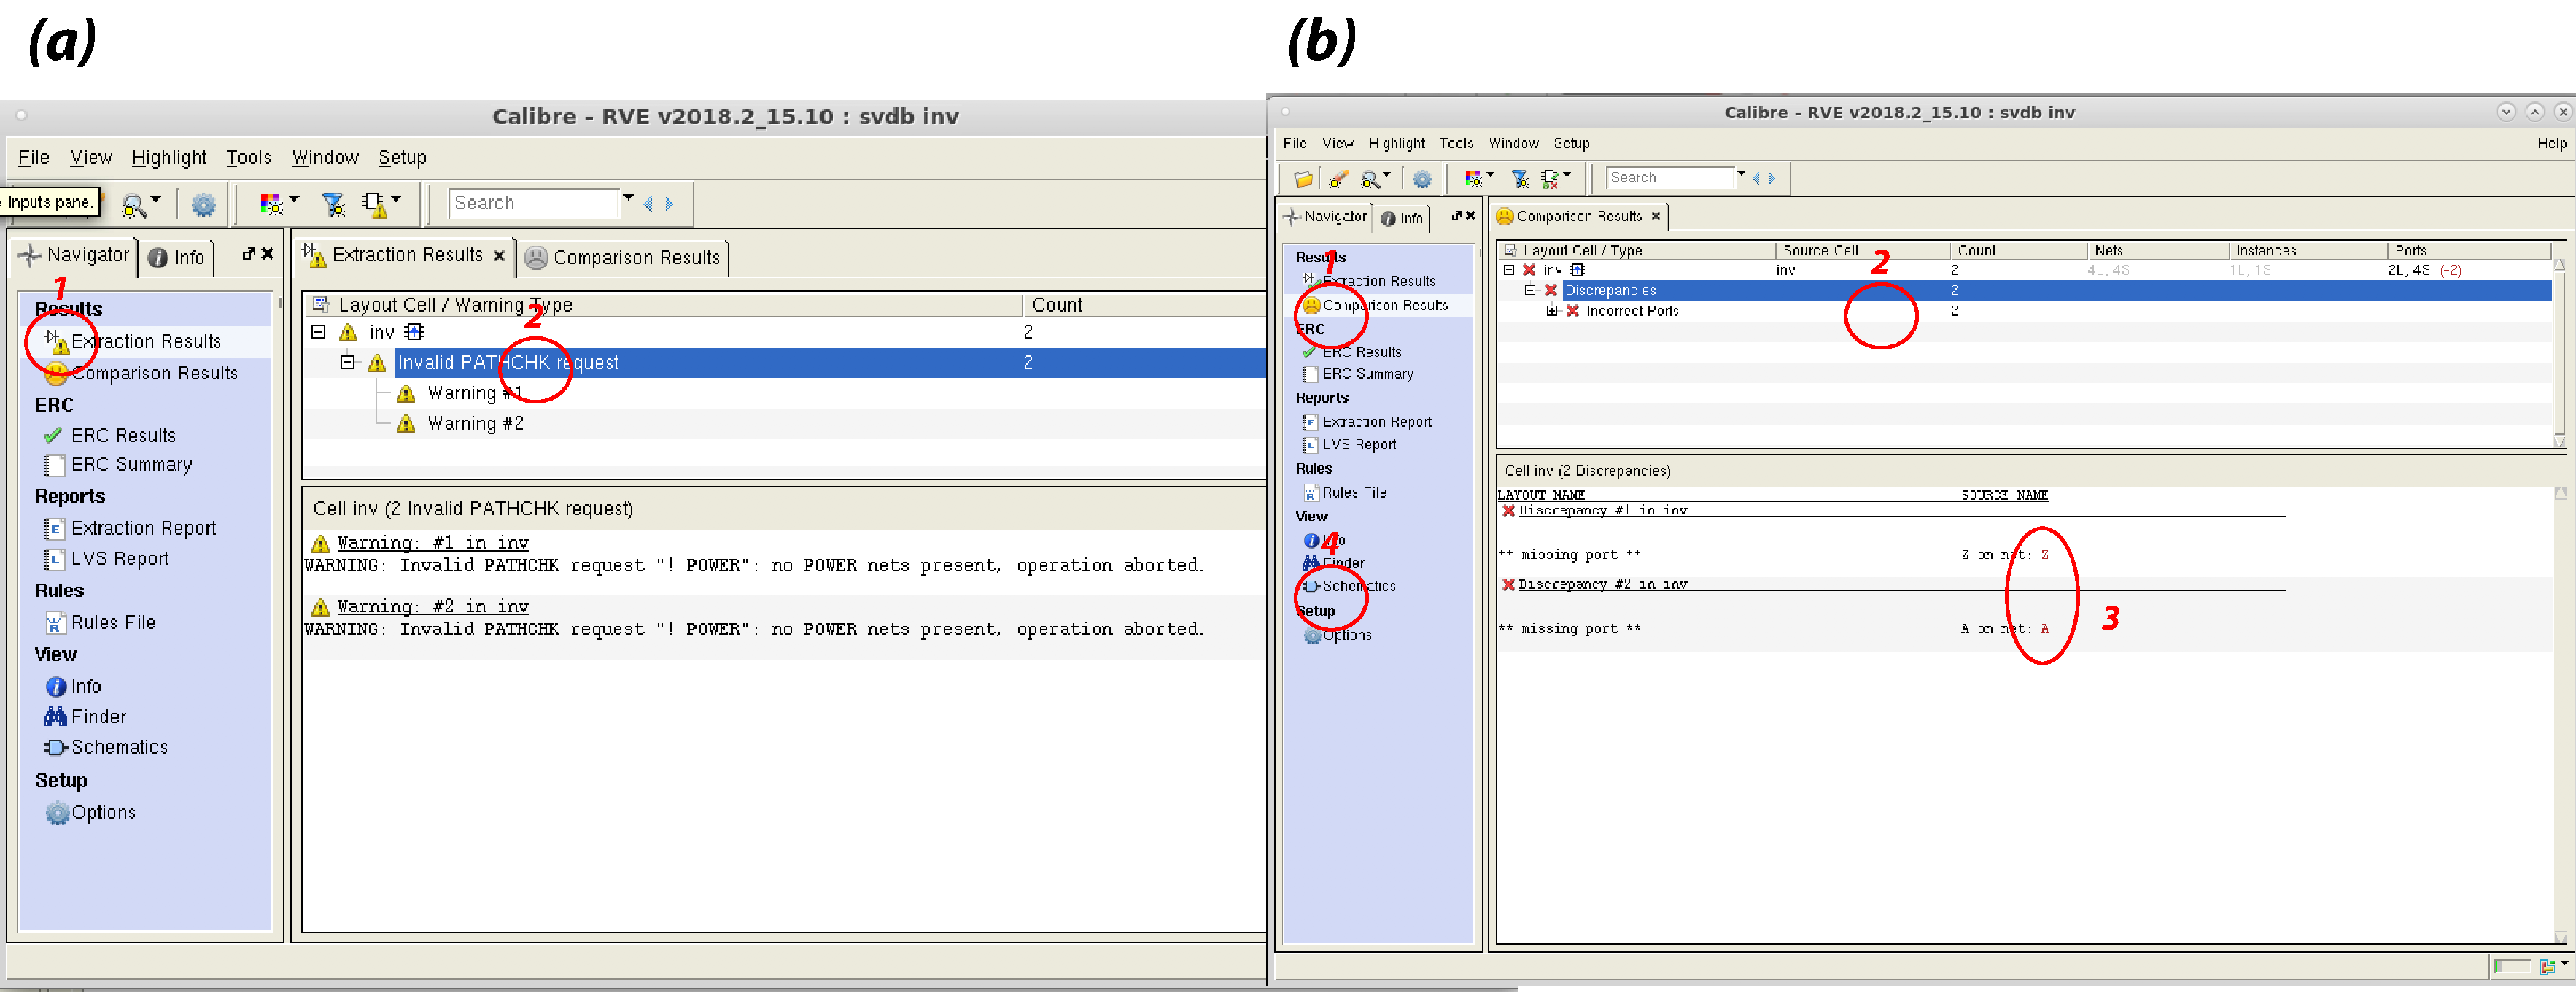
\includegraphics[scale=0.28]{figures/lab2_layout/bad_lvs}
	\caption{LVS result window for: (a) Extraction results; (b) Connectivity results.}
	\label{fig_lvs_bad}
\end{figure}

%\end{enumerate}

\begin{checkpoint}\label{check1}
	Please call an assistant and show him that your inverter design pass both the DRC and LVS with no errors.
\end{checkpoint}

\newpage 
\subsubsection{Parasitic Extraction (PEX)}
\begin{warning}
	The PEX step can only be done if your design is LVS compliant.
\end{warning}



\begin{figure}
	\vspace{-0mm}
	\centering
	\vspace{1cm}
	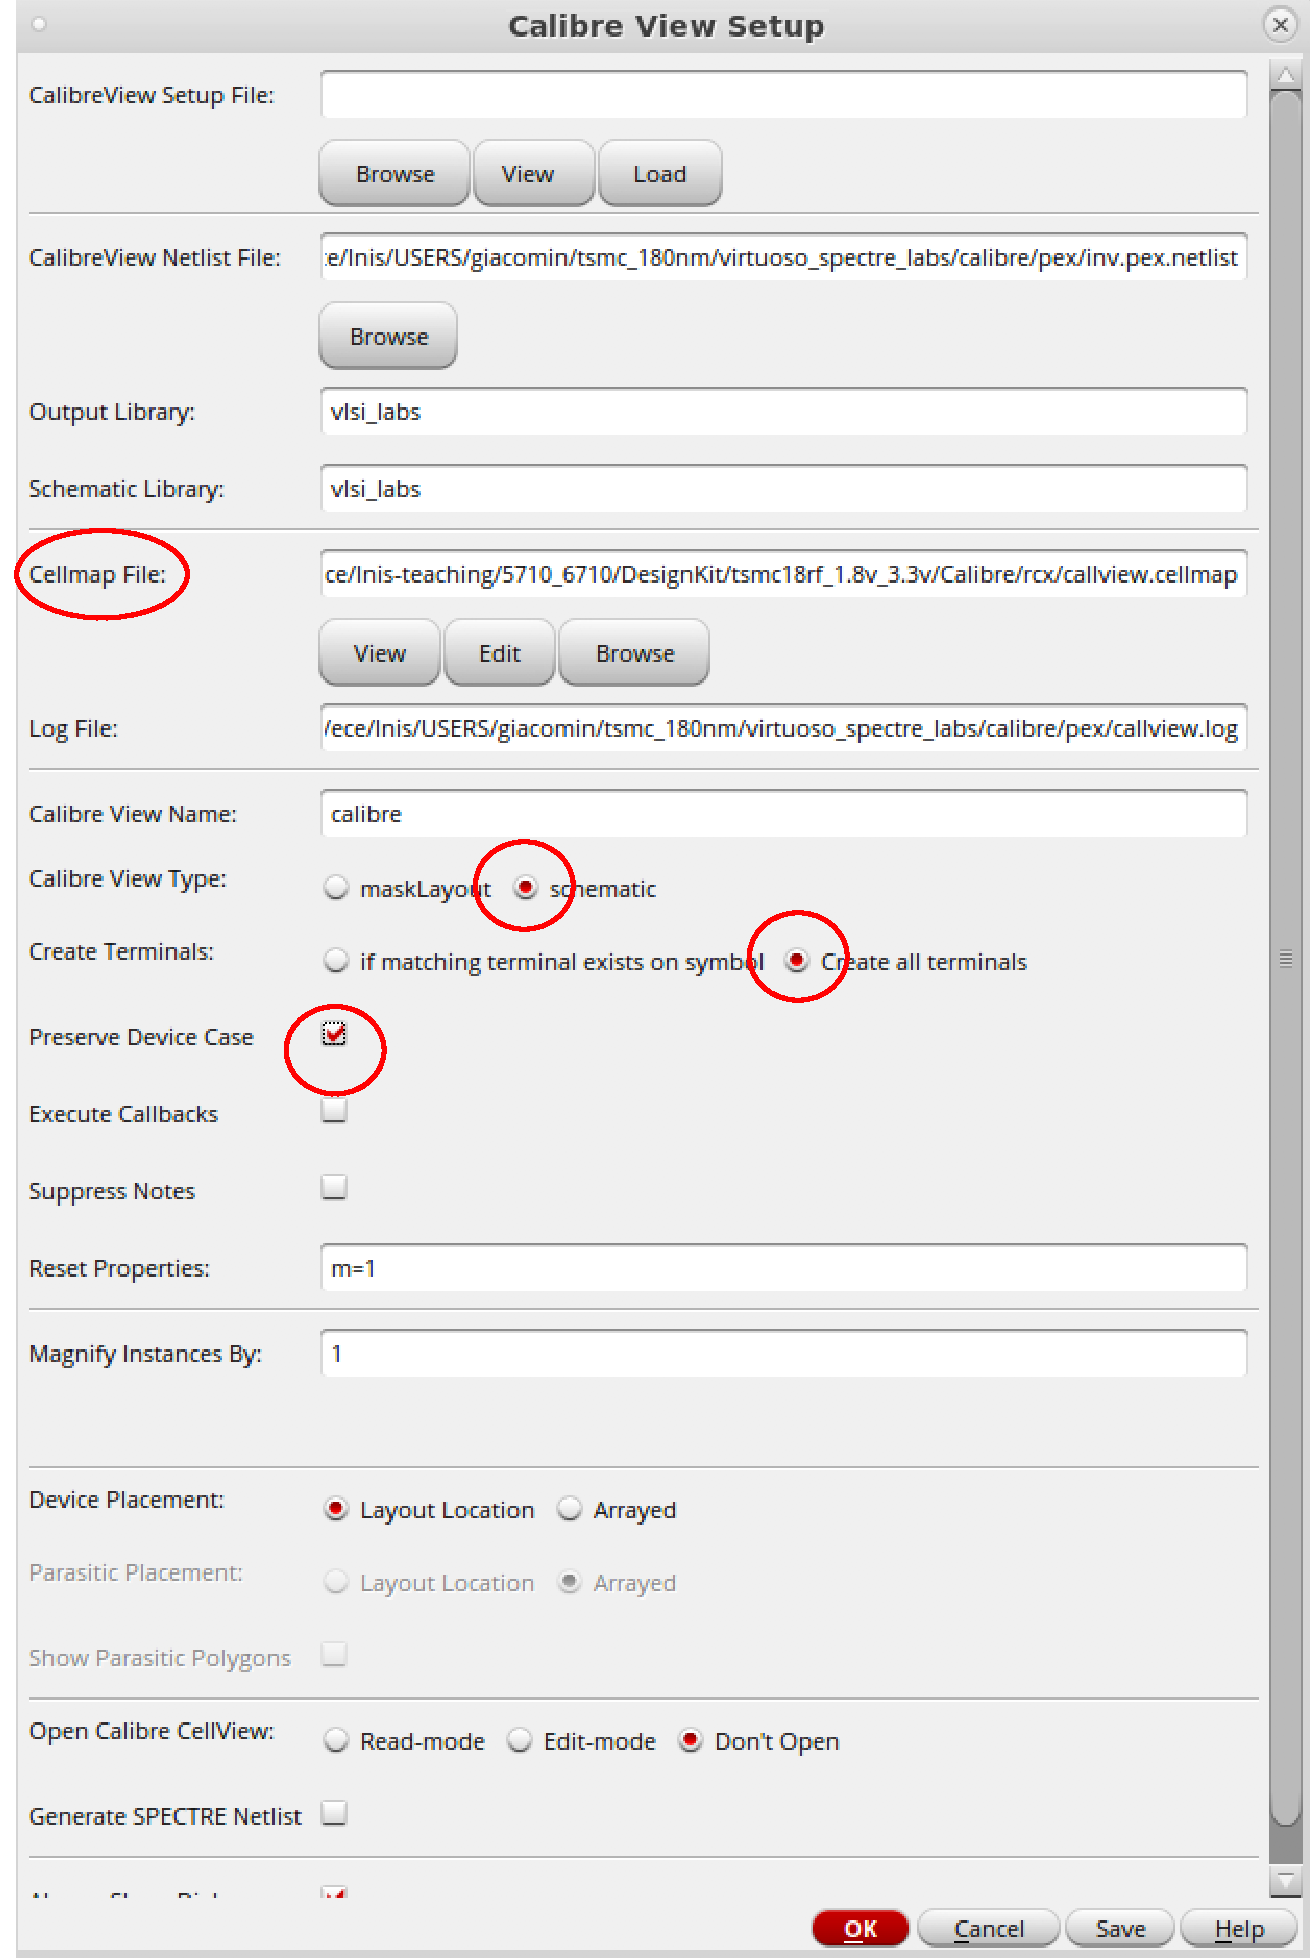
\includegraphics[scale=0.32]{figures/lab2_layout/pex_options.pdf}
	\caption{PEX options.}
	\label{fig_pex}
\end{figure}

\parbox[t]{\dimexpr\textwidth-\leftmargin}{%
	To perform the PEX step:
	\begin{enumerate}
		\item Launch the Calibre PEX tool: from the layout view: \textit{Calibre -> Run PEX…}.
		\item The Calibre PEX window now appears. Again, you normally should not have to modify any settings except setting the runset file to:
		
		\begin{codeline}
			/uusoc/facility/cad$\_$common/skywater-src-nda/s8/V2.0.1/PEX/xRC/Calibre$\_$PEX$\_$runset
		\end{codeline}

		\item Click on Run PEX.
		\item Then, a window will appear as depicted in Fig \ref{fig_pex}. Verify that the options (the important ones are highlighted in red) are the same as in Fig. \ref{fig_pex} (some fields, such as the library settings can of course differ depending on the name you chose).
		\item Click on $OK$ at the bottom of the window.
		\item You should get a pop-up window as shown in Fig. \ref{fig_pex_good} with no warnings.
		\item Once this is done, go back to the Library Manager window. You should be able to see a new view for your inverter cell in your working library named \textbf{calibre}. When you open it, you can see the resistances and capacitances modeling the parasitics of your layout.
		\begin{remark}
			Do not forget to check and save your calibre view (you might get some warnings but those are fine) before closing it. Otherwise, you will encounter an error when doing your post PEX simulation.
			\end{remark}
\end{enumerate}}

\begin{checkpoint}\label{check2}
	Please call an assistant and show him that the \textit{calibre} view for your inverter has been properly generated.
\end{checkpoint}


\begin{figure}[!h]
	\centering
	\includegraphics[scale=0.6]{figures/lab2_layout/pex_good}
	\caption{Successful PEX extraction.}
	\label{fig_pex_good}
\end{figure}

\subsection{CMOS Inverter Post Layout Simulation}
With technology scaling, the RC delay is now a big issue due to the increased parasitics. This is why it is important to perform a post layout simulation which takes into account the parasitics (after the PEX step). 
\begin{enumerate}
	\item Go to the library manager and open the schematic view of your inverter transient testbench ($inv\_testbench\_tran$).
	\item Launch ADE L. From the ADE window, open up the state you previously defined in the previous part: click on \textit{Session -> Load State ...}. A new window will appear, simply click on \textit{Ok}.
	\item Now, all the settings you previously defined (parameters values, analysis type, display output) should be there.
	\item To take into account the parasitics of your layout, we need to tell ADE to consider the parasitics in the simulation. To do so, go to the ADE window and go to: \textit{Setup -> Environment} and add the \textbf{calibre} view in first in the \textit{Switch View List}, as shown in Fig \ref{fig_simpex}.
	\item Click OK and launch the simulation. 
	\item Observe the output curves to check that your inverter behaves properly as well as how the delay changed compared the the simulation you ran before considering the parasitics.
	\begin{figure}[!h]
		\centering
		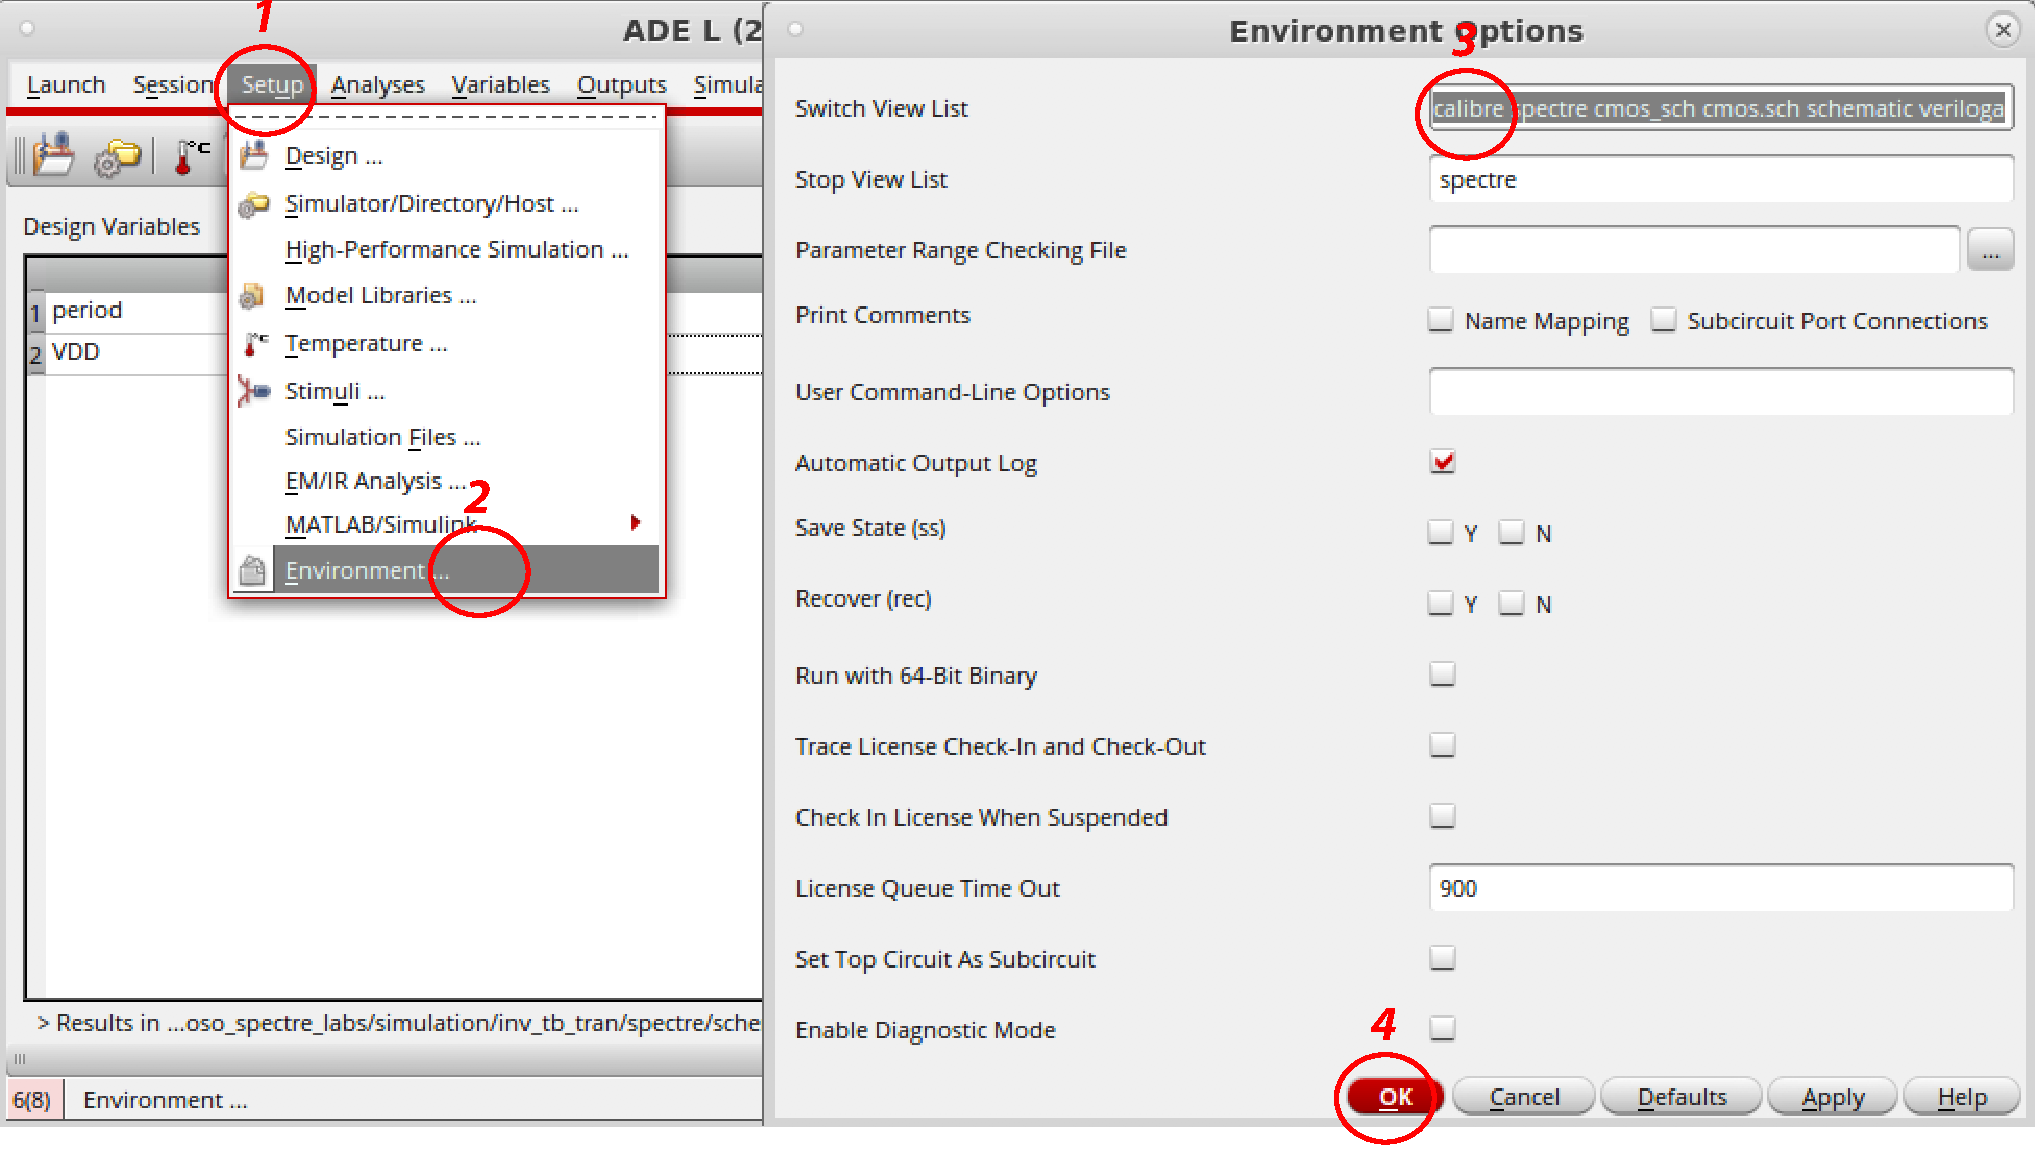
\includegraphics[scale=0.45]{figures/lab2_layout/ade_pex}
		\caption{ADE L environment options.}
		\label{fig_simpex}
	\end{figure}
	
	%\begin{remark}
	%	If you open the calibre view, you won't be able to save it because of a bug and you will not be able to run the simulation since you will get an error message saying that the calibre view is not saved. To be able to run the simulation by considering the calibre view, you will need to run the PEX again without opening the calibre view and then run your simulation.
	%\end{remark}
\end{enumerate}

	\begin{exercise}\ 
Report the rising, falling and propagation delays of your inverter after the PEX step. How did the delay change when compared to the pre-layout simulation? Why?		
\end{exercise}
\clearpage


\section{Assignment and Checkpoint Summary}
Write a report and answer the assignments asked during the lab, which are summarized below. Do not forget to validate the checkpoints, summarized below as well, by an assistant before the end of the lab.


	\begin{exercisesum}\	
			\vspace{-2mm}
	\begin{enumerate}
\item Report the rising, falling and propagation delays of your inverter after the PEX step. How did the delay changed when compared to the pre-layout simulation? Why?		
\item Provide a screenshot of the DRC result window as well as the LVS result window for the inverter, showing the correctness of your design.			
	\end{enumerate}
\vspace{-5mm}
\end{exercisesum}	

\begin{checkpointsum}\
	\vspace{-2mm}
		\begin{enumerate}
	\item Please call an assistant and show him that your inverter design pass both the DRC and LVS with no errors.
	\item Please call an assistant and show him that the \textit{calibre} view for your inverter has been properly generated.
		\end{enumerate}
	\vspace{-5mm}
\end{checkpointsum}




